\documentclass[crop, tikz, border=10pt]{standalone}

\begin{document}

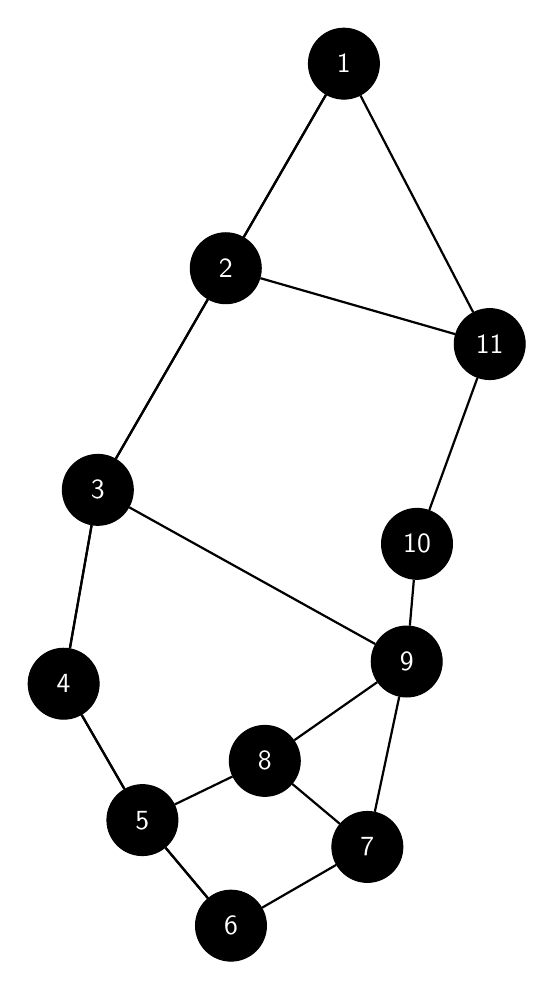
\begin{tikzpicture}[bn/.style={circle,fill,draw,text=white,font=\sffamily,minimum
size=9mm},every node/.append style={bn}]
 \path node (1) {1} -- ++ (-120:3) node (2) {2} -- ++(-120:3.25) node (3) {3}  -- ++(-100:2.5) node (4) {4} -- ++(-60:2) node (5) {5}
 -- ++ (-50:1.75) node (6) {6} -- ++ (30:2) node (7) {7} -- ++ (140:1.7) node (8) {8} -- ++ (35:2.2) node (9) {9} -- ++ (85:1.5) node (10) {10} -- ++ (70:2.7) node (11) {11};
\draw[thick] (1)--(2)--(3)--(4)--(5)--(6)--(7)--(8)--(9)--(10)--(11)--(1);
\draw[thick] foreach \X [count=\Y] in {2,...,6} {(\Y) -- (\X)} (2) -- (11) (3) -- (9) (5) -- (8) (7) -- (9);
\end{tikzpicture}

\end{document}